\documentclass[11pt,a4paper]{article}
\usepackage[utf8]{inputenc}
\usepackage[T1]{fontenc}
\usepackage{babel}
\babelprovide[import,main]{spanish}
\setlocalecaption{spanish}{table}{Tabla}
\usepackage{microtype}
\usepackage{lmodern}
\usepackage{amsmath,amssymb}
\usepackage{graphicx}
\usepackage{booktabs}
\usepackage{array}
\usepackage[margin=2.3cm]{geometry}
\usepackage[font=small,labelfont=bf]{caption}
\usepackage[hidelinks]{hyperref}

\newcommand{\ind}{\mathbb{1}}
\setlength{\parskip}{0.45em}
\setlength{\parindent}{0pt}

\begin{document}

% ------------------------------------------------------------------ Portada
\begin{titlepage}
\centering
\IfFileExists{logo_usa.png}{\includegraphics[width=4cm]{logo_usa.png}\par\vspace{1cm}}{}
{\Large\bfseries UNIVERSIDAD SERGIO ARBOLEDA\par}
\vspace{3cm}
{\LARGE\bfseries PREDICCIÓN DE CONGESTIÓN EN UN ENLACE:\\[0.3em]
CAPTURA DE TRÁFICO Y SELECCIÓN DE MODELO\par}
\vspace{2.5cm}
{\large INTELIGENCIA ARTIFICIAL\par}
\vspace{1.5cm}
{\large DOCENTE\\[0.3em] JOAQUÍN FERNANDO SÁNCHEZ CIFUENTES\par}
\vspace{1.5cm}
{\large ESTUDIANTE\\[0.3em]
JULIAN CAMILO CARO HERRERA\par}
\vfill
{\large NOVIEMBRE DE 2026\par}
\end{titlepage}

% ------------------------------------------------------------------ 1
\section{Montaje, cola y protocolo de captura}

\textbf{Topología.} El emisor A es Ubuntu 24.04 en WSL2 (kernel Linux, donde vive la
cola) y el receptor B es el anfitrión Windows con el servidor iperf3 3.22; los une el
conmutador virtual de Hyper-V. El profesor aceptó un montaje virtual. Lo que se mide
---los descartes de la cola configurada en la salida de A--- depende del kernel de A y
no del medio físico, y el enlace virtual tiene capacidad muy superior a la del cuello de
botella, como exige el enunciado. En la salida de A:
\texttt{tc qdisc replace dev eth0 root handle 10: tbf rate 10mbit burst 16kb limit 32kb}.

\textbf{Por qué WSL2 y no VirtualBox.} Se probó primero con dos VMs de VirtualBox. Con la
cola puesta y solo $4$~Mbit/s ofrecidos (menos de la mitad del límite) hubo entre 249 y
1\,276 descartes en 10~s, y la TBF registró 5\,919 \emph{overlimits}: ráfagas. El equipo
tiene Hyper-V forzado por la seguridad basada en virtualización y VirtualBox corre encima
de él; la VM se detiene $\approx$0,2~s, iperf3 recupera la tasa promedio enviando de golpe y la
ráfaga supera cubeta más cola. La etiqueta de congestión habría mezclado carga con
artefactos de la VM. En WSL2, que Hyper-V maneja directamente, la misma prueba dio
\textbf{0 descartes}.

\textbf{Límite efectivo y física de la cola.} Cada datagrama de 1200~B viaja en una trama de
$1200+8+20+14=1242$~B, que es lo que cuentan la TBF y \texttt{frame.len}. Con $C=10$~Mbit/s,
el límite en carga ofrecida por iperf3 es
\[
R^{*}=C\,\frac{1200}{1242}\approx 9{,}66\ \text{Mbit/s}.
\]
Verificación en los datos: en el escalón de 9,5~Mbit/s la tasa capturada tiene mediana
9,833~Mbit/s ($9{,}5\cdot1242/1200=9{,}83$). Si se ofrece $R>R^{*}$, la cubeta
($b=16\,384$~B) y la cola ($L=32\,768$~B) se agotan en
\begin{equation}
T_{\text{llenado}}(R)=\frac{b+L}{(1{,}035\,R-C)\cdot10^{6}/8},
\qquad
\delta(R)=\frac{(1{,}035\,R-C)\cdot10^{6}}{8\cdot1242}\ \text{descartes/s}.
\label{eq:llenado}
\end{equation}
\begin{table}[!htb]
\centering\small
\begin{tabular}{lcccccc}
\toprule
$R$ ofrecida (Mbit/s) & 10 & 10,5 & 12 & 14 & 20 & 30\\
\midrule
$T_{\text{llenado}}$ (s) & 1,12 & 0,45 & 0,16 & 0,088 & 0,037 & 0,019\\
$\delta(R)$ (descartes/s) & 35 & 87 & 244 & 452 & 1\,077 & 2\,119\\
\bottomrule
\end{tabular}
\caption{Ecuación~(\ref{eq:llenado}) para las tasas del calendario. Se verificó en el piloto (2\,222 descartes en 5~s a 14~Mbit/s; predicción 2\,260) y en prueba (figura~\ref{fig:magnitud}).}
\label{tab:llenado}
\end{table}

\textbf{Calendario.} La tabla~\ref{tab:llenado} fija el diseño. Una \emph{rampa}
($8\to9\to9{,}5\to10$ o $10{,}5\to$ tope) cruza el límite con un exceso pequeño: la cola
tarda 0,45--1,12~s en llenarse, así que la traza puede saturarse antes del primer descarte.
Un \emph{salto} desde la recuperación (4--6~Mbit/s) a 12, 14, 20 o 30~Mbit/s la llena en
menos de 0,16~s. Cada corrida tiene una fase base y pares rampa+salto en orden aleatorio
hasta $\approx$950~s de tráfico, con recuperaciones de 10--15~s; orden, tasas y duraciones se
sortean con semilla fija por corrida (\texttt{random.Random("congestion-cXX")}), de modo
que el calendario es reproducible y no lo elige a mano quien diseña. Así cada corrida
tiene $\approx$16 rampas y $\approx$16 saltos; con dos episodios por corrida, como sugiere el
enunciado, la prueba tendría $\approx$4 inicios. El calendario solo se usa para interpretar,
nunca como predictor.

\textbf{Captura.} Un script por corrida (\texttt{captura/corrida.sh}) arranca
\texttt{tcpdump}, muestrea \texttt{tc -j -s} cada 0,05~s sobre una grilla de tiempo fija
(el bucle con \texttt{sleep} del enunciado acumula atraso), ejecuta las fases de iperf3 y
anota hora y descartes de cada fase, todo con el reloj de A. Verificaciones en las seis
corridas: 0 descartes en todas las fases de base y recuperación, contador JSON igual al
\texttt{dropped} textual y 0 paquetes perdidos por el kernel.

\textbf{Pausas.} WSL2 se congela ocasionalmente: unas 30 veces por corrida, casi todas de
hasta $\approx$1~s, y una vez 30,7~s (c05) y 105~s (c06). Durante esas pausas la traza no tiene paquetes y después
no hay descartes en recuperación, así que fue la VM entera, sin ráfagas posteriores. Se
aplica la regla del enunciado: no se construyen filas que crucen una pausa ($\Delta>1{,}5$
periodos).

\begin{table}[!htb]
\centering\small
\begin{tabular}{llrrrrrr}
\toprule
Corrida & Rol & Fases & Tráfico (s) & Descartes & Pausas (tiempo) & Filas & Inicios\\
\midrule
c01 & entrenamiento & 129 & 988 & 243\,925 & 34 (26,5 s) & 10\,132 & 41\\
c02 & entrenamiento & 127 & 960 & 271\,445 & 34 (28,4 s) & 9\,961 & 40\\
c03 & entrenamiento & 131 & 975 & 221\,393 & 35 (29,4 s) & 9\,943 & 41\\
c04 & validación & 127 & 968 & 258\,694 & 31 (18,4 s) & 9\,789 & 38\\
c05 & prueba & 129 & 979 & 260\,935 & 33 (47,0 s) & 9\,839 & 42\\
c06 & prueba & 129 & 973 & 258\,745 & 33 (122,9 s) & 9\,789 & 39\\
\midrule
\multicolumn{6}{l}{Total} & 59\,453 & 241\\
\bottomrule
\end{tabular}
\caption{Corridas en orden de adquisición. \emph{Filas}: ventanas de 0,1~s utilizables (con rezagos y objetivo sin cruzar pausas). c06 se repitió con el mismo calendario tras una interrupción accidental.}
\label{tab:corridas}
\end{table}

% ------------------------------------------------------------------ 2
\section{Serie temporal y definición de congestión}

\textbf{Ventanas.} Con muestras de la cola en $t_0<t_1<\dots$ cada 0,05~s, la ventana $k$ es
$[t_{2k},t_{2k+2})$, de duración real $\Delta_k\approx0{,}1$~s, y
\[
r_k=\frac{8B_k}{10^{6}\Delta_k}\ \text{Mbit/s},\qquad n_k=\#\text{tramas},\qquad
d_k=D(t_{2k+2})-D(t_{2k}),
\]
con $B_k$ los bytes capturados y $D$ el contador acumulado de descartes. Se eligió
$\Delta=0{,}1$~s porque el profesor pidió más de 50\,000 datos: con ventanas de 1~s, las
seis corridas darían $\approx$6\,000 filas. Se descartó $0{,}05$~s porque a 10~Mbit/s un paquete
pesaría el 2~\% de $r_k$, justo la diferencia entre ``casi lleno'' (9,83) y ``lleno''
(10,0); con 0,1~s pesa el 1~\%. Inflar filas con ventanas solapadas se descartó porque
serían copias de la misma información.

\textbf{Congestión.} Definimos que el enlace está congestionado en la ventana $k$ si la cola
descartó al menos un paquete:
\[
C_k=\ind[d_k\ge1].
\]
Es lo que se mide directamente y corresponde a ``cuando los paquetes no pasan''. Las
alternativas consideradas coinciden con ella en casi todas las ventanas válidas: pérdida
de al menos 1~\% de lo enviado coincide en el 99,96~\%, y cola en saturación
($\text{overlimits}\ge1$) coincide en el 98,77~\% (738 ventanas saturadas aún sin pérdida;
ninguna con pérdida sin saturación). La razón está en la tabla~\ref{tab:llenado}: salvo
en el cruce de la rampa, la cola se llena en menos de una ventana, de modo que saturación
y pérdida casi siempre ocurren en la misma ventana. Ante definiciones equivalentes en los
datos, se eligió la más simple.

\textbf{Objetivo, alerta e inicio.} Al cierre de $k$ se predice $y_k=d_{k+1}$ y se alerta si
$\hat y_k\ge\tau$. El evento es $E_k=C_{k+1}$; un \emph{inicio} es $d_k=0\wedge d_{k+1}\ge1$.
Las entradas son las del enunciado, $x_k=(r_k,r_{k-1},r_{k-2},n_k)$. Como todas las tramas
miden 1242~B, $r_k\simeq0{,}009936\,n_k/\Delta_k$: $r$ y $n$ son casi colineales y sus
coeficientes no se pueden interpretar por separado, aunque las predicciones no se
afectan.

% ------------------------------------------------------------------ 3
\section{Modelos y selección}

Los tres modelos que el profesor pidió comparar predicen el mismo $y_k$ con las mismas
entradas y la misma regla de alerta, así que solo cambia el modelo. Para cada familia se
varía únicamente el hiperparámetro que controla su capacidad:
\begin{itemize}\itemsep0.2em
\item \textbf{Regresión lineal:} $\min_{\beta}\sum_k\bigl(y_k-\beta_0-\beta^{\top}x_k\bigr)^2$. No tiene hiperparámetro.
\item \textbf{Árbol de decisión} (CART de regresión): particiones de $x$ que minimizan el error cuadrático dentro de cada hoja, con profundidad $p\in\{1,\dots,12\}$.
\item \textbf{RNA (MLP):} ReLU y Adam, con entradas y salida estandarizadas con estadísticos de entrenamiento y parada temprana. Arquitecturas $(4)$, $(8)$, $(16)$ y $(16,8)$.
\end{itemize}
Se usaron Python, pandas y scikit-learn porque el enunciado los propone y porque
scikit-learn da a las tres familias la misma interfaz, lo que garantiza el mismo
protocolo para todas.

\textbf{Protocolo.} Cada candidato se entrena con c01--c03. En c04, el umbral se fija como
$\tau^{*}=\arg\max_\tau F_1(\tau)$ y gana el $F_1$ más alto. Se usa $F_1$ y no MAE porque
la alerta debe ser útil sobre \emph{cuándo} hay pérdida, no sobre \emph{cuánta}. c05--c06
se usan una sola vez, con todo ya fijado. Como referencias se incluyen la regla del
enunciado, $r_k\ge\tau_r$ (también ajustada en c04), y la \emph{persistencia},
$d_k\ge1$. Esta última usa el contador de la cola y no es un predictor desplegable; mide
qué parte del $F_1$ se obtiene con solo reconocer episodios que ya empezaron.

\begin{table}[!htb]
\centering\small\setlength{\tabcolsep}{4.5pt}
\begin{tabular}{llrrrrr}
\toprule
Modelo & Hiperparámetro & $\tau^{*}$ & Precisión & Sensibilidad & $F_1$ & Inicios anticipados\\
\midrule
Regresión lineal & --- & 44,29 & 0,959 & 0,967 & 0,963 & 18/38\\
\textbf{Árbol de decisión} & \textbf{profundidad 6} & \textbf{27,64} & \textbf{0,975} & \textbf{0,990} & \textbf{0,983} & \textbf{19/38}\\
RNA (MLP) & capas $(16,8)$ & 42,78 & 0,975 & 0,983 & 0,979 & 20/38\\
\midrule
Regla $r_k\ge\tau_r$ & --- & 9,907 & 0,958 & 0,986 & 0,972 & 21/38\\
Persistencia $d_k\ge1$ & --- & 1 & 0,989 & 0,989 & 0,989 & 0/38\\
\bottomrule
\end{tabular}
\caption{Validación (c04): mejor configuración de cada familia. Las profundidades 5 a 12 del árbol quedan a menos de 0,002 de $F_1$ (unas 10 ventanas mal clasificadas de 9\,789), así que la profundidad no es crítica.}
\label{tab:validacion}
\end{table}

Se elige el \textbf{árbol de profundidad 6}. La tabla~\ref{tab:validacion} adelanta el
resultado principal: la persistencia supera a todos los modelos en $F_1$ sin anticipar un
solo inicio. Los $F_1$ globales miden sobre todo la capacidad de reconocer episodios en
curso.

% ------------------------------------------------------------------ 4
\section{Resultados en prueba (c05--c06)}

\begin{table}[!htb]
\centering\small
\begin{tabular}{lrrrrrrrr}
\toprule
Modelo & MAE & VP & FP & FN & VN & Precisión & Sensibilidad & $F_1$\\
\midrule
\textbf{Árbol (prof.\ 6)} & 21,13 & 6\,915 & 166 & 74 & 12\,473 & 0,977 & 0,989 & 0,983\\
RNA $(16,8)$ & 22,51 & 6\,859 & 164 & 130 & 12\,475 & 0,977 & 0,981 & 0,979\\
Regresión lineal & 28,55 & 6\,732 & 259 & 257 & 12\,380 & 0,963 & 0,963 & 0,963\\
Regla $r_k\ge9{,}907$ & --- & 6\,890 & 272 & 99 & 12\,367 & 0,962 & 0,986 & 0,974\\
Persistencia & 0,84 & 6\,908 & 82 & 81 & 12\,557 & 0,988 & 0,988 & 0,988\\
\bottomrule
\end{tabular}
\caption{Prueba: 19\,628 ventanas; MAE en paquetes por ventana de 0,1~s (las salidas negativas se llevan a 0). Matriz de confusión del evento ``habrá descarte en $k+1$''.}
\label{tab:prueba}
\end{table}

\begin{table}[!htb]
\centering\small
\begin{tabular}{lcccc}
\toprule
Modelo & Rampa: cruce (31) & Rampa: reinicio tras pausa (18) & Salto (32) & Total (81)\\
\midrule
\textbf{Árbol (prof.\ 6)} & 30 & 11 & 2 & 43 (53~\%)\\
RNA $(16,8)$ & 31 & 0 & 4 & 35 (43~\%)\\
Regresión lineal & 31 & 6 & 2 & 39 (48~\%)\\
Regla $r_k\ge9{,}907$ & 31 & 6 & 4 & 41 (51~\%)\\
Persistencia & 0 & 0 & 0 & 0\\
\bottomrule
\end{tabular}
\caption{Inicios anunciados al cierre de $k$, sobre el total de inicios evaluables en prueba. \emph{Reinicio tras pausa}: la cola se vacía durante los $\approx$0,2~s entre dos comandos de iperf3 dentro de una rampa y vuelve a descartar al empezar el tope.}
\label{tab:inicios}
\end{table}

\begin{figure}[!htb]
\centering
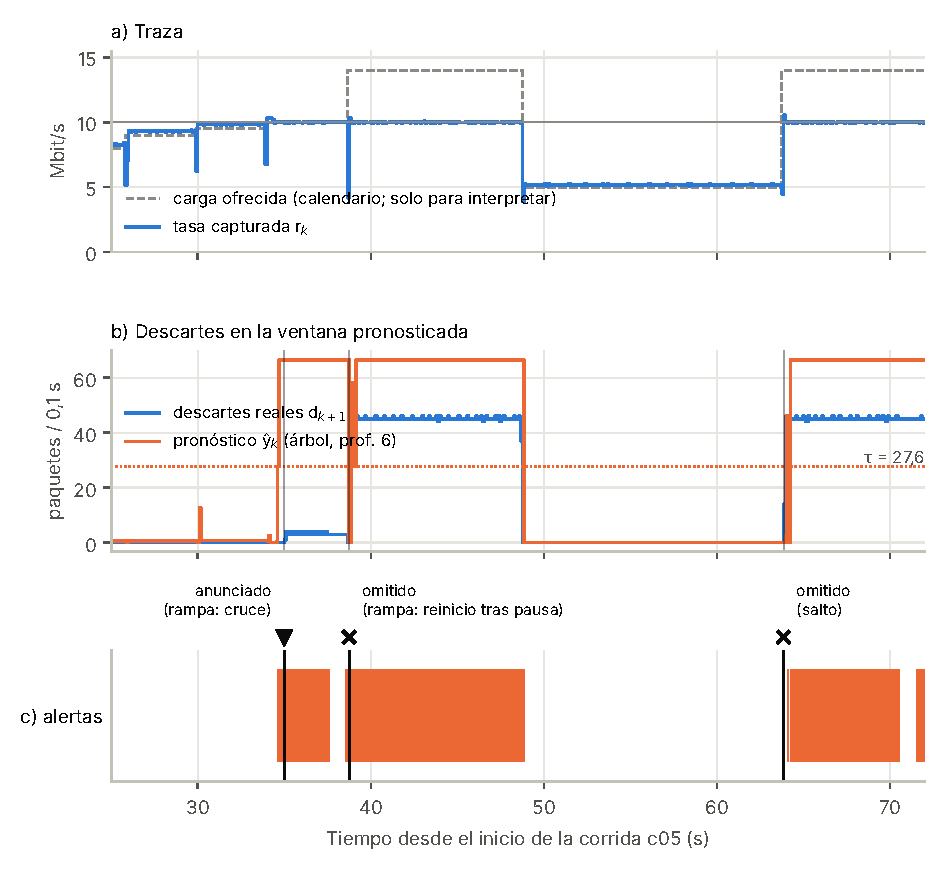
\includegraphics[width=0.9\linewidth]{figuras/fig2_serie_prueba.pdf}
\caption{Corrida c05, 25--72~s, con paneles alineados. Cada pronóstico se dibuja en la ventana a la que se refiere ($k+1$). Hay una rampa cuyo cruce se anuncia (35,0~s), un reinicio tras la pausa entre comandos que se omite (38,7~s) y un salto a 14~Mbit/s que se omite (63,8~s). La alerta que empieza en 34,7~s cuenta como falsa para el horizonte de 0,1~s, aunque precede al inicio por 0,3~s.}
\label{fig:serie}
\end{figure}

% ------------------------------------------------------------------ 5
\section{Discusión}

\textbf{¿El modelo anticipó inicios o reconoció episodios en curso?} En prueba hay 6\,908
ventanas de persistencia por cada 81 inicios. Por eso el $F_1$ global (0,983) refleja casi
solo la persistencia: la regla trivial $d_k\ge1$ obtiene 0,988 y no anticipa nada. Sobre
los inicios, el árbol anuncia 43 de 81, pero el promedio esconde dos comportamientos
opuestos (tabla~\ref{tab:inicios}): anuncia 30 de 31 cruces de rampa y solo 2 de 32
saltos. Anticipa cuando la carga sube gradualmente; ante un salto, solo reconoce el
episodio una ventana después.

\textbf{Rampas frente a saltos.} La figura~\ref{fig:tasas} lo explica con la
tabla~\ref{tab:llenado}. En un cruce de rampa a 10~Mbit/s la cola tarda 1,12~s en
llenarse. Durante ese tiempo la salida ya está en el límite: en la ventana previa al
inicio, $r_k>9{,}9$ en el 100~\% de los casos, frente al 2~\% de las ventanas normales. En
un salto la cola se llena en $\le0{,}16$~s, y la ventana previa casi siempre está en la
tasa de recuperación (mediana 5,2~Mbit/s; $r_k>9{,}9$ solo en el 16~\%). La única señal
que conserva la traza es que la salida esté saturada, y en un salto la saturación y la
pérdida llegan juntas.

\begin{figure}[!htb]
\centering
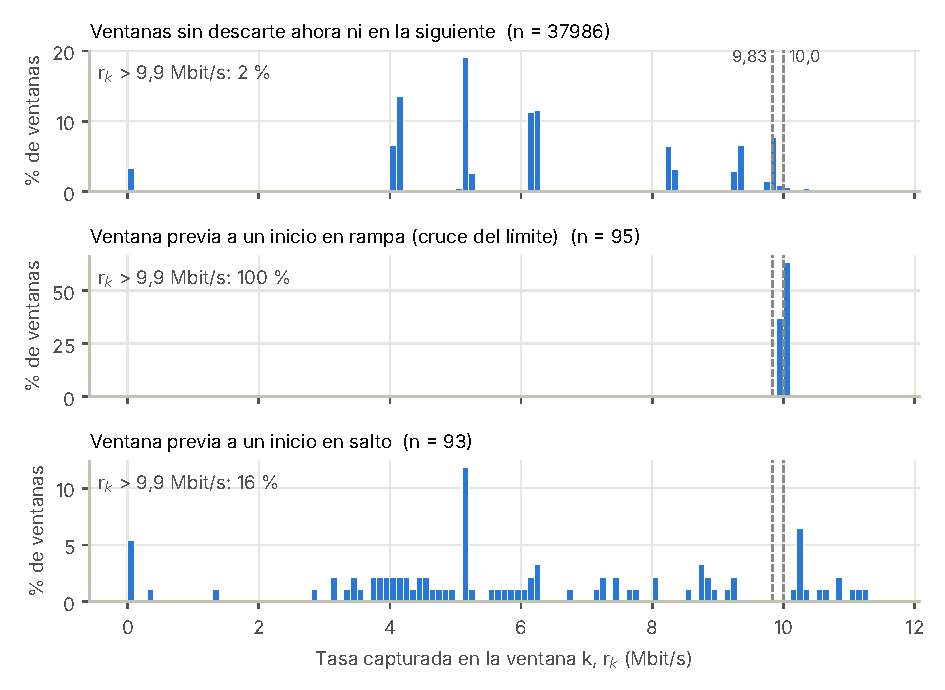
\includegraphics[width=0.8\linewidth]{figuras/fig1_tasa_antes_de_inicio.pdf}
\caption{Distribución de $r_k$ en las seis corridas (descriptiva; la selección y la evaluación usan solo c04 y c05--c06).}
\label{fig:tasas}
\end{figure}

\textbf{Una falsa alarma.} De las 166 falsas alarmas del árbol, 112 ocurren en escalones de
9,5--10,5~Mbit/s, antes del primer descarte. De las 130 que ocurren con $d_k=0$, 111
anteceden a un descarte en los 3~s siguientes (mediana: 0,40~s después). Son anticipos que
el horizonte de 0,1~s cuenta como error, como la alerta de 34,7~s en la
figura~\ref{fig:serie}: la cola se estaba saturando y perdió paquetes 0,3~s después. Otras
36 ocurren al final de un episodio: el generador deja de enviar y nada en la traza lo
anuncia.

\textbf{Un inicio omitido.} En el salto a 14~Mbit/s de 63,8~s (figura~\ref{fig:serie}), la
ventana previa tiene $r_k=5{,}17$, la recuperación. Según la tabla~\ref{tab:llenado}, la
cola se llena en 0,088~s, dentro de la propia ventana del salto, así que no había nada que
ver. El omitido de 38,7~s es de otro tipo: durante los $\approx$0,2~s entre dos comandos de iperf3,
$r_k$ cae a $\approx$4~Mbit/s y la cola se vacía. Es un artefacto del generador, no un cambio de
carga, y explica 18 de los 81 inicios de prueba.

\textbf{Qué limita la predicción cuando la carga cambia sin aviso.} La traza se toma
\emph{después} de la cola, y eso impone dos límites:
\begin{itemize}\itemsep0.2em
\item \textbf{No ve la magnitud.} La salida satura en 10~Mbit/s ofrezca uno 12 o 30. En
las ventanas de persistencia, los descartes reales siguen la ecuación~(\ref{eq:llenado})
(de 3,5 a 211,8 por ventana; figura~\ref{fig:magnitud}), mientras el árbol predice $\approx$66 en
todos los casos. De ahí un MAE de $\approx$21 paquetes por ventana, frente a 0,84 de la
persistencia, que sí lee el contador.
\item \textbf{No ve un salto antes de la pérdida.} Antes de ella no queda rastro en la
traza. Por eso los tres modelos y la regla $r_k\ge9{,}907$ anuncian los mismos cruces
(30--31 de 31). El árbol gana en $F_1$ (0,983 frente a 0,974) porque emite menos falsas
alarmas que la regla (166 frente a 272), no porque anticipe más.
\end{itemize}
La regresión lineal es la más débil ($F_1=0{,}963$, MAE 28,5): la relación entre $r_k$ y
$d_{k+1}$ es un escalón (casi cero bajo 10~Mbit/s, grande en la saturación), y la recta
($\hat\beta_r=14{,}1$) solo la aproxima.

\begin{figure}[!htb]
\centering
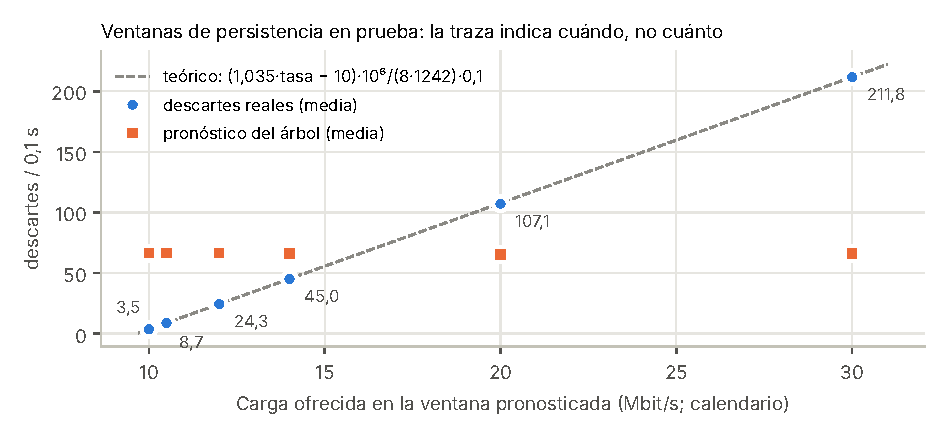
\includegraphics[width=0.85\linewidth]{figuras/fig3_magnitud.pdf}
\caption{Ventanas de persistencia en prueba, agrupadas por la carga ofrecida (calendario).}
\label{fig:magnitud}
\end{figure}

\textbf{Limitaciones.}
\begin{itemize}\itemsep0.2em
\item El montaje es virtual (WSL2 y Windows). Sus pausas ocuparon $\approx$4~\% del tiempo de captura y obligaron a excluir el 1,3~\% de las ventanas.
\item La selección se hizo con una sola corrida de validación.
\item Las pausas entre comandos de iperf3 generan reinicios que no son cambios reales de carga.
\item Con un horizonte de una ventana (0,1~s), parte de las ``falsas'' alarmas son anticipos reales.
\end{itemize}

\end{document}
